\documentclass[12pt,openright,
chapter=TITLE, % títulos de capítulos convertidos em letras maiúsculas
section=TITLE, % títulos de seções convertidos em letras maiúsculas
subsection=title, % títulos de subseções convertidos em letras maiúsculas
%fleqn, %fórmulas são vistas alinhadas pela esquerda ao invés de centralizadas. 
oneside,a4paper,english,french,spanish]{abntex2}

\usepackage{cmap}	
\usepackage{lmodern}	
\usepackage[T1]{fontenc}	
\usepackage[utf8]{inputenc}		
\usepackage{lastpage}		
%\usepackage{indentfirst}
\usepackage{color}	
\usepackage{graphicx}	
\usepackage{units}
\usepackage[alf,bibjustif,recuo=0.0cm]{abntex2cite} % bibjustif justifica a referência.
\usepackage[brazilian,hyperpageref]{backref}
\usepackage{bold-extra}
\usepackage{eso-pic}










\input{fixos/comandos}
\newcommand{\curso}[1]{\def\imprimircurso{#1}}

\newcommand{\departamento}[1]{\def\imprimirdepartamento{#1}}
\newcommand{\Title}[1]{\def\imprimirTitle{#1}}


\newcommand{\palavraChaveUm}[1]{\def\imprimirpalavrachaveum{#1}}
\newcommand{\palavraChaveDois}[1]{\def\imprimirpalavrachavedois{#1}}
\newcommand{\palavraChaveTres}[1]{\def\imprimirpalavrachavetres{#1}}
\newcommand{\palavraChaveQuatro}[1]{\def\imprimirpalavrachavequatro{#1}}

\newcommand{\palavraChaveUmingles}[1]{\def\imprimirpalavrachaveumingles{#1}}
\newcommand{\palavraChaveDoisingles}[1]{\def\imprimirpalavrachavedoisingles{#1}}
\newcommand{\palavraChaveTresingles}[1]{\def\imprimirpalavrachavetresingles{#1}}
\newcommand{\palavraChaveQuatroingles}[1]{\def\imprimirpalavrachavequatroingles{#1}}


\newcommand{\cdu}[1]{\def\nomecdu{#1}}
\newcommand{\dataDaAprovacao}[1]{\def\imprimirdatadaaprovacao{#1}}

\newcommand{\mes}[1]{\def\imprimirmes{#1}}

\newcommand{\dia}[1]{\def\imprimirdia{#1}}

\newcommand{\publicacao}[1]{\def\imprimirpublicacao {#1}}

\newcommand{\ENDERECO}[1]{\def\imprimirendereco{#1}}

\newcommand{\CEP}[1]{\def\imprimirCEP{#1}}


\newcommand{\membroConvidadoUm}[1]{\def\imprimirmembroconvidadoum{#1}}
\newcommand{\membroConvidadoDois}[1]{\def\imprimirmembroconvidadodois{#1}}
\newcommand{\membroCoorientador}[1]{\def\imprimirmembroCoorientador{#1}}


\newcommand\BackgroundPic{%
	\put(0,0){%
		\parbox[b][\paperheight]{\paperwidth}{%
			\vfill
%			\centering
%			\includegraphics[width=\paperwidth,height=\paperheight,%
%				keepaspectratio]{figuras/capa.eps}%
			\vfill
		}
	}
}

\renewcommand{\imprimircapa}{%
  \begin{capa}
    \center
    \vspace*{0in}
	{\textbf{\imprimirinstituicao}}
	\par
	{\textbf{\imprimirdepartamento}}

	\vspace{2. in}
	{\textbf{\large \imprimirtitulo}}
    	\vspace{0.25 in}
    	\par
         {\textbf{\large \imprimirautor}}
    	\vspace{2. in}

	    \textbf{ORIENTADORA: \imprimirorientador}\\
    	    \textbf{COORIENTADORA: \imprimirmembroCoorientador}\\
   	    \vspace{0.5 in}
	    \textbf{DISSERTAÇÃO DE MESTRADO EM ENGENHARIA BIOMÉDICA}
		
    \vspace*{1.0 in}
    \textbf{PUBLICAÇÃO: \imprimirpublicacao / \imprimirdata }
    \par
    \textbf{\imprimirlocal: \imprimirmes\,-\,\imprimirdata}  
  \end{capa}
}


% Dados pessoais
\autor{NOME DO ESTUDANTE}
\departamento{PROGRAMA DE PÓS-GRADUAÇÃO EM ENGENHARIA \\ BIOMÉDICA}
\instituicao{UnB - UNIVERSIDADE DE BRASÍLIA 
		\par
		FGA - FACULDADE UNB GAMA}
		
\local{BRASÍLIA/DF}
\data{2015}
\mes{MÊS }
\dia{DIA}

% Dados do trabalho
\titulo{TÍTULO}
\Title{TITLE}

\orientador{Dr(a).}
\membroCoorientador{Dr(a).}
\membroConvidadoUm{Dr(a).}
\membroConvidadoDois{Dr(a).}

\palavraChaveUm {Palavra chave um}
\palavraChaveDois {Palavra chave dois}
\palavraChaveTres {Palavra chave três}
\palavraChaveQuatro {Palavra chave quatro}

\palavraChaveUmingles {Key-words-1}
\palavraChaveDoisingles {Key-words-2}
\palavraChaveTresingles {Key-words-3}
\palavraChaveQuatroingles {Key-words-4}
% Configurações de aparência do PDF final
% alterando o aspecto da cor azul
\definecolor{black}{RGB}{0,0,0}

% informações do PDF
\makeatletter
\hypersetup{
     	%pagebackref=true,
		pdftitle={\@title}, 
		pdfauthor={\@author},
    	pdfsubject={\imprimirpreambulo},
	    pdfcreator={LaTeX with abnTeX2},
		pdfkeywords={abnt}{latex}{abntex}{abntex2}{trabalho acadêmico}, 
		colorlinks=true,       		% false: boxed links; true: colored links
    	linkcolor=black,          		% color of internal links
    	citecolor=black,        		% color of links to bibliography
    	filecolor=magenta,      		% color of file links
		urlcolor=black,
		bookmarksdepth=4
}
\makeatother
% O tamanho do parágrafo é dado por:
\setlength{\parindent}{1.25cm} % Controle do espaçamento entre um parágrafo e outro.

\setlength{\parskip}{0.2cm}  % tente também \onelineskip

% Remova o comentário abaixo para espaçamento simples
%\SingleSpacing

%\setlength{\mathindent}{0.6cm} % Altera o recuo das equações de tiver o pacote fleqn em documentclass

\counterwithout{equation}{chapter} %Faz com que as equações sejam numeradas 1,2,3,...

\counterwithout{table}{chapter} %Faz com que as equações sejam numeradas 1,2,3,...


\counterwithout{footnote}{chapter} %Faz com que as notas de rodapé sejam numeradas 1,2,3,...

%\setlength\afterchapskip{\baselineskip} % Espaçamento entre o título e o texto

\renewcommand{\ABNTEXchapterfontsize}{\fontsize{14}{14}\selectfont} %Letra e tamnaho da fonte do sumário
\renewcommand{\ABNTEXsectionfontsize}{\fontsize{14}{14}\selectfont}
\renewcommand{\ABNTEXsubsectionfontsize}{\fontsize{14}{14}\selectfont}



\makeindex

\begin{document}
\frenchspacing 
\imprimircapa

\begin{folhadeaprovacao}
\begin{center}
    \vspace*{0in}
	{\textbf{\imprimirinstituicao}}
	\par
	{\textbf{\imprimirdepartamento}}

	\vspace{0.5 in}
	{\textbf{\large \imprimirtitulo}}
    	\vspace{0.25 in}
    	\par
         {\textbf{\large \imprimirautor}}
    	\vspace{0.25 in}
\end{center}
\textbf{DISSERTAÇÃO DE MESTRADO SUBMETIDA AO PROGRAMA DE PÓS-GRADUAÇÃO EM ENGENHARIA BIOMÉDICA DA FACULDADE GAMA DA
UNIVERSIDADE DE BRASÍLIA, COMO PARTE DOS REQUISITOS NECESSÁRIOS PARA A OBTENÇÃO DO GRAU DE MESTRE EM
ENGENHARIA BIOMÉDICA.}
\flushleft	
	\vspace{0.5 in}    
    \textbf{APROVADO POR:}\\
    \vspace{0.5 in}    
    \rule{10cm}{.1mm}\\
    {\textbf{Prof. \imprimirorientador} \\ \textbf{(Orientadora)} }\\
    \vspace{0.5 in}    
   \rule{10cm}{.1mm}\\ 
   {\textbf{Prof. \imprimirmembroCoorientador} \\ \textbf{(Co-Orientadora)}}\\
    \vspace{0.5 in}    
   \rule{10cm}{.1mm}\\
    {\textbf{Prof. \imprimirmembroconvidadodois} \\ \textbf{(Examinador Externo)}}\\
    
    \end{folhadeaprovacao}

\begin{resumo}

\begin{center}
\textbf{\imprimirtitulo}
\end{center}

\begin{flushleft}
\footnotesize
\textbf{Autor: \imprimirautor }\\
\textbf{Orientadora: Profa. \imprimirorientador }\\
\textbf{Coorientadora: \imprimirmembroCoorientador} \\
\textbf{Programa de Pós-Graduação em Engenharia Biomédica} \\
\textbf{\imprimirlocal \imprimirdata }
\end{flushleft}

O presente trabalho tem como objetivo implementar um software como serviço, para análise e simulação de marcha humana, baseado num modelo arquitetural em camadas. 
A grande vantagem de tal software é sua disponibilidade via \emph{web} e até mesmo em dispositivos móveis. 
Com esta disponibilidade e o uso crescente do software, surge a possibilidade da geração de uma base de dados com dados de marcha humana. 
O sistema ainda conta com um módulo de simulação, que tirará proveito desta base. 
A análise de movimento baseada em dados espaciais, recuperadas de um software de \emph{motion capture}, foi implementada e simulação de sinais usando a rede neural artificial CMAC também.
O projeto é \emph{open source} e funcionalidades novas serão adicionadas frequentemente.  

\vspace{\onelineskip}
    
 \noindent
 \textbf{Palavras-chaves}: \imprimirpalavrachaveum, \imprimirpalavrachavedois, 
			    \imprimirpalavrachavetres, \imprimirpalavrachavequatro.
\end{resumo}


\begin{resumo}[Abstract]
 \begin{otherlanguage*}{english}

 \begin{center}
\textbf{\imprimirTitle}
\end{center}

\begin{flushleft}
\footnotesize
\textbf{Author: \imprimirautor}\\
\textbf{Supervisor: Prof. \imprimirorientador} \\
\textbf{Co-supervisor: \imprimirmembroCoorientador} \\
\textbf{Post-Graduation Program in Biomedical Engineering} \\
\textbf{Brasília, Month of Year.}\newline
\end{flushleft}
 
Texto corrido sem parágrafo. 1 página.

   \vspace{\onelineskip}
 
   \noindent 
   \textbf{Key-words}: 	\imprimirpalavrachaveumingles, \imprimirpalavrachavedoisingles, 
			\imprimirpalavrachavetresingles, \imprimirpalavrachavequatroingles.
 \end{otherlanguage*}
\end{resumo}


\input{fixos/indiceAutomatico}
\pdfbookmark[0]{\listtablename}{lot}
\listoftables*
\cleardoublepage


\renewcommand*\listfigurename{Lista de Figuras}
\pdfbookmark[0]{\listfigurename}{lof}
\listoffigures*
\cleardoublepage

\begin{siglas}
	\item[ACM DL] \emph{Association from Computer Machinery Digital Lybrary]}
	\item[API] \emph{Application Program Interface}
	\item[CAPES] \emph{Coordenação de Aperfeiçoamento de Pessoal de Nível Superior}
	\item[CPD] Centro de Processamento de Dados
	\item[BSON] \emph{Binary Object Notation} 
	\item[CSS] \emph{Cascade Style Sheet}
	\item[FCE] Faculdade Ceilândia 
	\item[FGA] Faculdade Gama
	\item[HTML] \emph{HiperText Markup Language}
	\item[HTTP] \emph{HiperText Transfer Protocol}
	\item[GNU] GNU is Not Unix
	\item[GUGT] \emph{Get Up and Go Test}
	\item[IEEE] \emph{Institute of Electrical and Electronics Engineers}
	\item[IMU] \emph{Inertial Measurement Unit}
	\item[JSON] \emph{JavaScript Object Notation} 
	\item[LIS] Laboratório de Informática em Saúde
	\item[LPH] Laboratório de Performance Humana
	\item[MIT]  \emph{Massachusetts Institute of Technology}
	\item[MLP] \emph{Multi Layer Perceptron}
	\item[MOCAP] \emph{Mootion Capture}
	\item[MVC] \emph{Model View Controller}
	\item[PCA] \emph{Principal Component Analysis}
	\item[QTM] \emph{Qualisys Track Manager}
	\item[RNA] Rede Neural Artificial
	\item[REST] \emph{Representational State Transfer}
	\item[SPA] \emph{Single-Page Applications}
	\item[SVM] \emph{Suport Vector Machine}
	\item[UnB] Universidade de Brasília
	\item[URL] \emph{Uniform Resource Locator}
	\item[VM] \emph{Virtual Machine}

\begin{comment}
\item[AC]  Aquisição do Conhecimento
\item[ACM] \textit{Association for Computing Machinery}
\item[ACR] \textit{American College of Radiology}
\item[BI-RADS] Sistema de Laudos e Registros de Dados de Imagens da Mama
\item[caBIG]  \textit{Cancer Biomedical Informatics Grid}
\item[CADe] \textit{Computer-aided Detection}
\item[CADx]  \textit{Computer-aided Diagnosis}
\item[CAE]  Controle Automático de Exposição
\item[CAR]  \textit{Computer-Assisted Radiology}
\item[CC] Incidência Craniocaudal
\item[CDA]  \textit{HL7 Clinical Document Architecture}
\item[CBEB]  Congresso Brasileiro de Engenharia Biomédica
\item[CEN]  \textit{Comité Européen de Normalisation}
\item[CMS]  \textit{Clinical Management System}
\item[CRT]  \textit{Cathode-Ray Tube}
\item[DICOM] \textit{Digital Imaging Communications in Medicine}
\item[DIN/PACS]  \textit{Installation Site for Digital Imaging Network and PACS}
\item[DMWL] \textit{DICOM Modality Worklist}
\item[EC]  Elicitação de Conhecimento
\item[FDA]  \textit{Food and Drug Administration}
\item[FFDM] \textit{Full-field Digital Mammography}
\item[HIMSS] \textit{Healthcare Information and Management Systems Society}
\item[HIS]  \textit{Hospital Information System}
\item[HL7] \textit{Health Level 7}
\item[IBICT]  Instituto Brasileiro de Informações em Ciência e Tecnologia
\item[IEEE] \textit{Institute of Electrical and Electronics Engineers}
\item[IHE]  \textit{Integrating the Healthcare Enterprise}
\item[IMAC] \textit{Image Management and Communication}
\item[INCA] Instituto Nacional de Câncer
\item[IOD] \textit{Information Objects Definition}
\item[LCD] \textit{Liquid Crystal Display}
\item[MC]  Mamografia Convencional
\item[MD]  Mamografia Digital
\item[MG]  \textit{Digital Mammography X-Ray Image}
\item[MLO]  Incidência Médio-Lateral Oblíqua
\item[MPPS]  \textit{Modality Performed Procedure Step}
\item[NBIA] \textit{National Biomedical Imaging Archive}
\item[NCBI] \textit{National Center for Biotechnology Information}
\item[NEMA] \textit{National Electrical Manufacturers Association} \item[NLM]  \textit{National Library of Medicine}
\item[PACS]  \textit{Picture Archiving and Communications Systems}
\item[PMBOK]  \textit{Project Management Body of Knowledge}
\item[PRINCE2] \textit{Process-Based Method for Effective Project Management}
\item[RAID] \textit{Redundant Array of Independent Drives}
\item[RIS]  \textit{Radiology Information Systems}
\item[RSNA] \textit{Radiological Society of North America}
\item[SCP]  \textit{Service Class Provider}
\item[SCU]  \textit{Service Class User}
\item[SOP]  \textit{Service-Object Pair}
\item[SUS]  Sistema Único de Saúde
\item[TI] Tecnologia da Informação
\item[USP] Universidade de São Paulo
\item[UFSC] Universidade Federal de Santa Catarina
\end{comment}

\end{siglas}

\begin{simbolos}
	\item \textbf{Símbolos Latinos}
	  \item[$F_1$, $F_2$] Força ($N$)

    \begin{comment}
	  \item[$C_H$] Coeficiente de altura de carga (-)
	  \item[$C_Q$] Coeficiente de vazão (-)
	  \item[$C_P$] Coeficiente de potência (-)
	  \item[$D$] Dimensão linear característica, diâmetro ($m$)
	  \item[$g$] Aceleração gravitacional ($m\cdot s^{-2}$)
	  \item[$G$] Grau de reação (-)
	  \item[$h$] Altura da carga hidráulica no vertedor ($m$)
	  \item[$h_1, h_2, h_3$] Perda de carga ($m$)
	  \item[$h_v$] Pressão de vapor da água ($mca$)
	  \item[$H$] Altura Líquida de carga, altura de queda líquida ($m$)
	  \item[$H_d$] Queda disponível na entrada da turbina ($m$)
	  \item[$H_r$] Queda disponível na saída da turbina ($m$)
	  \item[$H_s$] Altura de sucção ($m$)
	  \item[$n$] Rotação da turbina (rpm)
	  \item[$n_s$] Rotação específica (rpm)
	  \item[$P_a$] Pressão atmosférica ($Pa$)
	  \item[$P_1$, $P_2$] Pressão ($Pa$)
	  \item[$P_e$] Potência de Eixo ($W$)
	  \item[$P_h$] Potência hidráulica ($W$)
	  \item[$Q$] Vazão volumétrica ($m^3\cdot s^{-1}$)
	  \item[$r$] Raio ($m$)
	  \item[$R_e$] Número de Reynols (-)
	  \item[$u$] Velocidade média do fluido ($m\cdot s^{-1}$)
	  \item[$v_1, v_2, v_3$] Velocidade média nas sessões 1, 2 e 3 ($m\cdot s^{-1}$) 
	  \item[$z_1$, $z_2$] Nível topográfico ($m$)

	  
	\item \textbf{Símbolos Gregos}
	  
	  
	  \item[$\alpha$] Medida angular ($^o$)
	  \item[$\gamma$] Peso específico ($N\cdot m^{-3}$)   
	  \item[$\delta X$] Incerteza de uma grandeza X (-)
	  \item[$\eta$] Rendimento total (-)
	  \item[$\eta_h$] Rendimento hidráulico (-)
	  \item[$\theta$] Medida angular ($^o$)

	  \item[$\nu$] Coeficiente de viscosidade cinemática ($m^2\cdot s^{-1}$)
	  \item[$\rho$] massa específica ($kg\cdot m^{-3}$)
	  \item[$\sigma$] Coeficiente de cavitação (-)
	  \item[$\psi$] Desvio padrão amostral (-)
	  \item[$\tau$] Torque ($N\cdot m$)
	  \item[$\omega$] Velocidade angular ($rad\cdot s^{-1}$)
	  \item[$\Pi_1, \Pi_2, \Pi_3$] Grupos pi do \textit{Teorema Pi de Buckingham}
  \end{comment}  
 
  
\end{simbolos}
 

\textual

\pagestyle{simple} % Bordo superior da página apenas com a numeração da página.
\chapter[INTRODUÇÃO]{\textbf {Introdução}}
\section{CONTEXTUALIZAÇÃO E FORMULAÇÃO DO PROBLEMA}
Quando o autor deparou-se com um problema na área de análise de marcha, 
ele seguiu toda uma metodologia para resolver este problema. 
Ao ler artigos desta área, notou que muitas das atividades que ele realizou, provavelmente foram realizadas por aqueles autores também. 
Na época o autor estava desenvolvendo um software simulador de um joelho, que poderia ser implantado num sistema embarcado para controle de uma possível prótese transfemural ativa.
A metodologia usada naquele trabalho pode ser resumida da seguinte forma:
\begin{enumerate}
	\item Coletar dados de movimentos usando marcadores passivos fixados no corpo de um paciente. Os dados eram coletados por uma série de câmeras;
	\item Usar o software \emph{Qualisys Track Manger (QTM)} \cite{Qualisys2010} para converter os dados para o formato \emph{MATLAB}, assim era possível manipulá-los;
	\item Criar um programa para extrair os dados em formatos mais amigáveis à sua manipulação;
	\item Fazer cálculos de ângulos, velocidades angulares, posicionamentos dos marcadores, velocidades dos marcadores;
	\item Fazer gráficos de toda essa informação. Lembrando, tudo isso usando \emph{MATLAB};
	\item Persistir toda essa informação para uso futuro;
	\item Criar um algoritmo complexo, que usa certos dados como entrada e algum outro como saída;
	\item Executar várias simulações alterando vários parâmetros até achar uma combinação de parâmetros que simule o sinal de uma forma desejada.
\end{enumerate}

Várias das etapas acima, poderiam ser desenvolvidas num software com interface gráfica, facilitando e muito o trabalho do pesquisador da área de análise de marcha. Por exemplo, o novo software receberia o arquivo do \emph{QTM}, criaria todos os dados de movimentos citados automaticamente colocando-os numa base de dados e permitiria imprimir gráficos de todos eles.

Este foi o contexto inicial, que impulsionou o desenvolvimento deste trabalho,
mas além deste problema notou-se um potencial a mais, o \emph{QTM} que é o software 
de captura de dados. Ele é muito bom mas é de uso genérico. Para utilizá-lo como 
software de análise de marcha, há um trabalho grande a ser feito. O indício disto é 
que a maioria dos pesquisadores com que o pesquisador teve contato no laboratório, 
usavam o mesmo processo, coletavam com o \emph{QTM} e processavam com o \emph{MATLAB}. 
Geralmente, a outra opção é usar softwares de análise de marcha específicos como 
o software \emph{Kin Trak} e \emph{Ortho Trak}, descritos em \citeonline{Moraes2003}. Além disso todos, esses softwares, inclusive o
\emph{QTM}, são softwares \emph{desktop}, que possuem licenças caríssimas, o que limita o
uso dos dados pelos pesquisadores, que tem que ir ao laboratório ou ter um computador
com uma licença válida. Daí surgiu outra oportunidade, isto é, criar o novo software 
como um serviço na \emph{web}, que pode ir evoluindo ao longo do tempo, ou seja,
recebendo adições de funcionalidades constantemente, até que seja bom o suficiente
para ser usado por qualquer profissional de saúde no globo.
Para que a evolução seja constante, optou-se por adotar metodologias ágeis que privilegiem a mudança contínua e o incremento iterativo de funcionalidades.

Com o poder de processamento dos dispositivos móveis de hoje, a nova
aplicação também pode resolver problemas de mobilidade, pois pode disponibilizar dados de pacientes
onde e quando o profissional de saúde quiser.


\section[OBJETIVOS]{OBJETIVOS}

\subsection[Objetivo Geral]{\textbf{Objetivo Geral}}
O presente trabalho visa iniciar um projeto de desenvolvimento de software como serviço, para análise e simulação de marchar humana.

\subsection[Objetivo Específicos]{\textbf{Objetivos Específicos}}
Os objetivos específicos são:
\begin{itemize}
	\item Definir um processo de desenvolvimento ágil adequado ao projeto;
	\item Explicitar uma visão arquitetural inicial do software;
	\item Escolher componentes de software a serem usados na solução;
	\item Criar um \emph{backlog} inicial de histórias de usuários;
	\item Selecionar um conjunto mínimo de histórias de usuários, suficientes para uma \emph{release} funcional do software;
	\item Implementar e testar estas histórias de usuários.
\end{itemize}

\section[REVISÃO DA LITERATURA]{revisão da literatura}



\chapter[FUNDAMENTAÇÃO TEÓRICA]{\textbf {fundamentação teórica}}
\section[MAMOGRAFIA DIGITAL]{MAMOGRAFIA DIGITAL}
\subsection[Mamografia e o câncer de mama]{\textbf{Mamografia e o câncer de mama}}

Segundo o INCA (Instituto Nacional de Câncer), “o número de casos novos de câncer de
mama esperados para o Brasil em $2010$ será de $49.240$, com um risco estimado de $49$ casos
a cada $100$ mil mulheres”. Essa estatística confirma que o câncer de mama é o segundo
tipo de câncer mais freqüente no mundo e o mais comum entre as mulheres. A cada ano,
cerca de $22\%$ dos novos casos de câncer em mulheres são de mama e por isso, os governos
do mundo inteiro têm investido em políticas para a detecção precoce da doença \cite{inca}. $\ldots$

A equação da continuidade na forma diferencial, presente na Eq. (\ref{cont}), representa o
princípio de conservação da massa em um escoamento e um exemplo de equação em LaTeX.
Onde $\rho$ é a densidade, $t$ é o tempo e $\vec{u}$ a velocidade do fluido.
\begin{equation}
\label{cont}
\frac{\partial \rho}{\partial t} + \nabla \ldotp (\rho \vec{u}) 
\end{equation}

\chapter[METODOLOGIA]{\textbf {metodologia}}

\section[AMBIENTE DE ESTUDO]{AMBIENTE DE ESTUDO}

Como este trata de um projeto de desenvolvimento de software na área de análise de marcha, dois ambientes de trabalho distintos foram amplamente utilizados. São estes:

\begin{enumerate}
	\item Laboratório de Informática em Saúde (LIS) na Faculdade Gama (FGA) da Universidade de Brasília (UnB);
	\item Laboratório de Performance Humana (LPH) na Faculdade Ceilândia (FCE) da UnB.
\end{enumerate}

No LIS foram desempenhadas as tarefas relativas a engenharia de software e disponibilização do software.
Foram utilizadas estações de trabalho do tipo \emph{Power Mac} com sistema operacional \emph{MAC OS X} 10.10.3, sendo que uma foi preparada para funcionar como servidor de aplicação e roteador de rede. 
A estação preparada, serve de hospedeira de duas máquinas virtuais (\emph{Virtual Machines} - VMs) rodando através do software \emph{Virtualbox} 4.3. 
Cada VM utiliza sistema operacional \emph{Debian Wheezy GNU/Linux}. 
Uma destas VMs foi configurada como roteador e \emph{firewall} e a outra como servidor de aplicações.  
Outra estação de trabalho \emph{Power Mac} idêntica e um notebook rodando \emph{Ubuntu 14.04 GNU/Linux} foram utilizados como máquinas de desenvolvimento.
Um diagrama da rede criada no LIS é mostrado na figura \ref{lis_rede}.

\begin{figure}[ht]
	\centering
	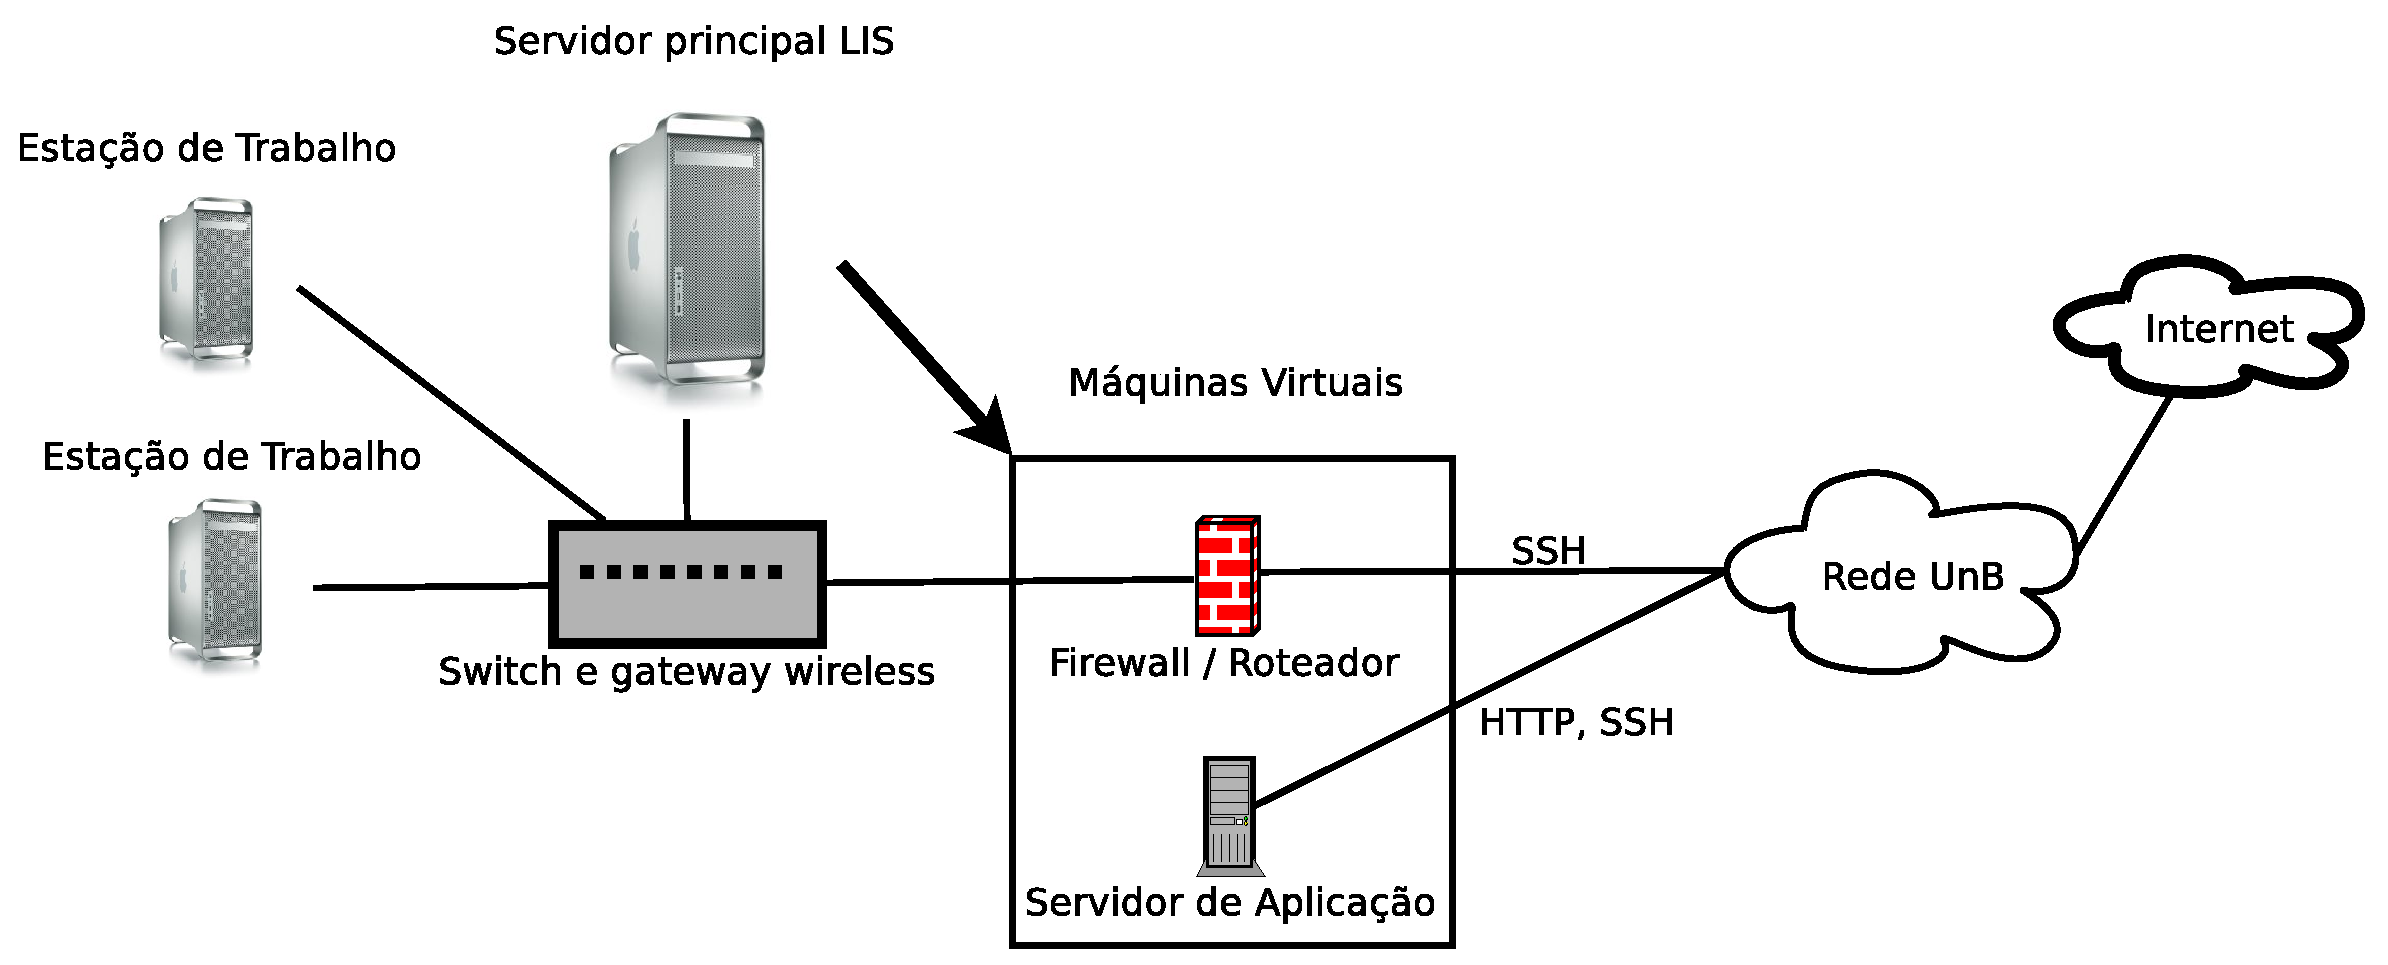
\includegraphics[width=15cm]{figuras/lis_rede.eps}
	\caption{Rede LIS}
	\label{lis_rede}
\end{figure}

O LPH foi utilizado para captura de dados de marcha humana. Este laboratório está equipado para coletar dados de plataformas de força, eletromiógrafos e de marcadores posicionados no corpo do paciente através de câmeras de vídeo (\emph{Motion Capture} - MOCAP). Para este trabalho foi utilizado o software \emph{QTM 3.2} da \emph{Qualisys}. 

\section[DELIMITAÇÃO DO ESTUDO]{DELIMITAÇÃO DO ESTUDO}

Este trabalho tem como foco estabelecer uma metodologia de desenvolvimento inicial a um sistema de análise e simulação de marcha. 
Ele não busca ser extensivo o suficiente para criar um produto pronto para o mercado, mas pretende, através da implementação de funcionalidades reais, estabelecer uma arquitetura mínima e funcional que sirva de base para a construção do sistema. 
Como consequência, o projeto também integra os principais componentes desta arquitetura, por exemplo, o serviço de banco de documentos, com a \emph{Application Program Interface} (API) \emph{web}.
Um software como este, robusto o suficiente para ser viável no mercado, seria muito caro. 
Por exemplo, um desenvolvedor sênior no mercado de Brasília, não custaria menos de R\$ 100.000,00 por ano para uma empresa. 


\section[VISÃO]{VISÃO} 
Apesar deste trabalho ter um objetivo específico e delimitado, dele nasce um projeto maior, cuja visão é o desenvolvimento de um software como serviço para análise e simulação de marcha, utilizando o estado da arte em técnicas para este fim. 
O software deve ser construído utilizando-se métodos ágeis e terá uma arquitetura adaptável que permita evolução contínua.

A estratégia é lançar a versão inicial do software como projeto de código livre, conseguir parceiros e procurar um modelo de negócio sustentável para mantê-lo.

\section[MODELO DE GESTÃO]{MODELO DE GESTÃO}
O software terá um modelo de gestão baseado no método \emph{SCRUM}, como definido em \ref{scrum_sec}.
O método não é adotado na plenitude, sendo adaptado segundo as limitações de recursos do projeto.

Nesta fase inicial, o processo conta com um desenvolvedor, que também assume o papel de \emph{scrum master}, e um \emph{product owner}. 
Devido ao tamanho reduzido da equipe e da localização distinta dos membros, não há \emph{daily scrum}, mas problemas de trabalho cotidianos são resolvidos por telefone, \emph{email} ou mensagens instantâneas. 

O princípio de \emph{time boxing} é mantido. Ficou definido que o \emph{sprint} consiste do prazo de duas semanas. Ao final do \emph{sprint} uma reunião em duas fases é realizada. A primeira fase consiste na revisão do \emph{sprint} anterior. Já a segunda fase é o planejamento do próximo \emph{sprint}.

Um \emph{backlog} de produto é mantido. Na reunião de final de \emph{sprint} é criado um \emph{backlog} de \emph{sprint}. 
Os itens de \emph{backlog} são mantidos na forma de estórias de usuários, conforme \ref{user_stories_sec}.
Na Figura \ref{scrum_projeto} é apresentada a visão geral do processo.

\begin{figure}[ht]
	\centering
	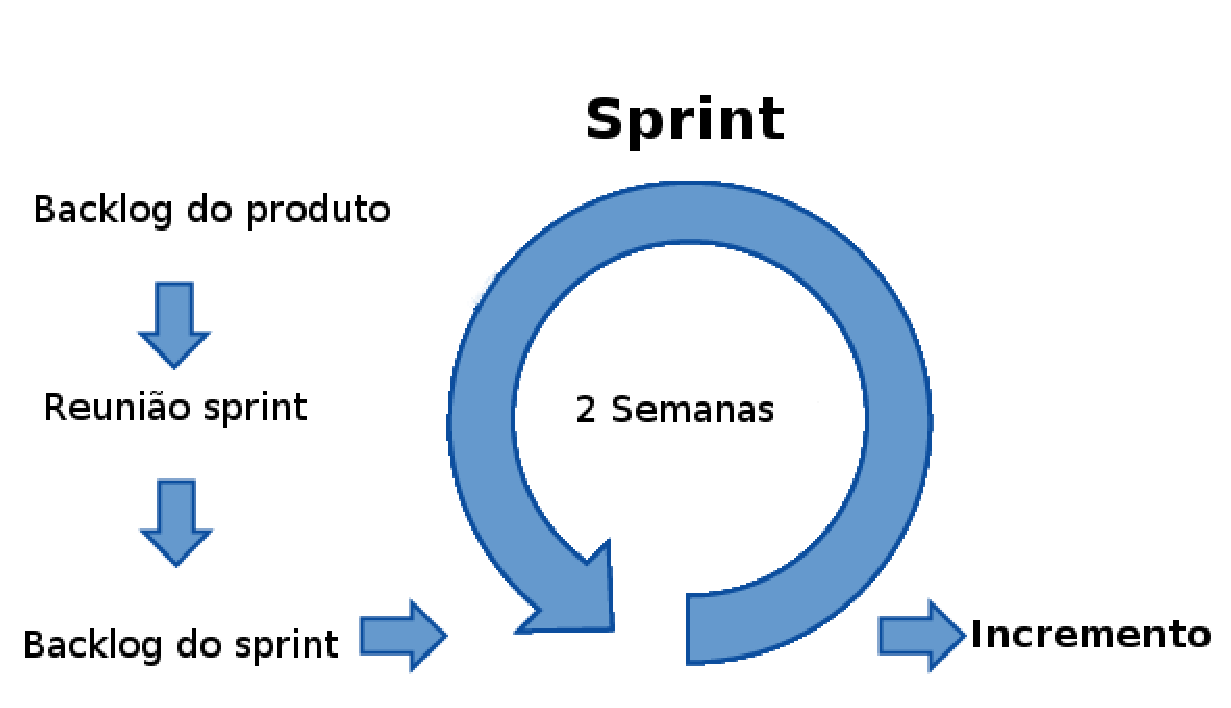
\includegraphics[width=15cm]{figuras/scrum_projeto.eps}
	\caption{Processo de desenvolvimento.}
	\label{scrum_projeto}
\end{figure}






\section[MODELO DE ARQUITETURA]{MODELO DE ARQUITETURA}

O modelo de arquitetura no seu nível mais elevado, pode ser visto como um modelo de três camadas, conforme a Figura \ref{camadas_arquitetura}.
\begin{figure}[ht]
	\centering
	\includegraphics[width=7cm]{figuras/camadas.eps}
	\caption{Camadas arquiteturais.}
	\label{camadas_arquitetura}
\end{figure}

A camada \emph{web} é responsável pela interação com o usuário. 
A camada \emph{Web API} é responsável pela lógica de negócio. 
A camada de base de documentos é responsável pela persistência dos dados da aplicação.


\subsection[CAMADA DE APLICAÇÃO WEB] {CAMADA DE APLICAÇÃO WEB}
Esta camada foi projetada para rodar em \emph{browsers} que suportam \emph{HTML} 5. 
Ela é desenvolvida usando-se \emph{Javascript}, \emph{CSS} e \emph{HTML}. 
Além disso, adotou-se o \emph{framework} de desenvolvimento \emph{web} \emph{AngularJS}, ver \ref{angularjs}. 

Como o projeto não possuía recursos adequados a criação de uma equipe de desenvolvimento \emph{web} completa, afim de se minimizar os problemas com \emph{design web}, optou-se por usar a biblioteca \emph{angular-material}, ver \ref{angular_material}. 

A Figura \ref{material_amostra}, mostra um exemplo de uma tela criada com as diretivas do angular-material. Note que todo o \emph{look and feel} da tela é determinado pelo comportamento padrão da biblioteca.

\begin{figure}[H]
	\centering
	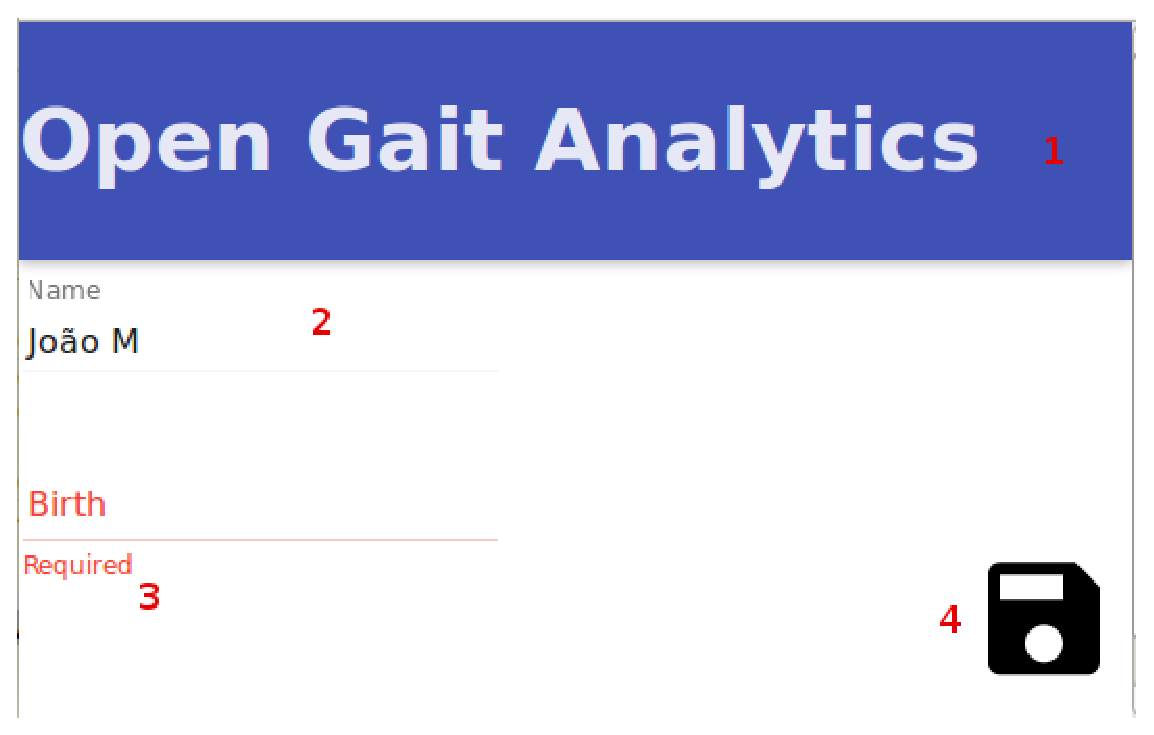
\includegraphics[width=9cm]{figuras/material_amostra.eps}
	\caption[Exemplo de uma tela criada com \emph{angular-material}.]{Exemplo de uma tela criada com \emph{angular-material}. 1) Diretiva \emph{md-toolbar}; 2) Diretiva \emph{md-input-container}; 3) Diretiva \emph{ng-messages} em conjunto com a \emph{md-input-container}; 4) Diretiva \emph{md-button}.}
	\label{material_amostra}
\end{figure}

\textbf{ORGANIZAÇÃO DO CÓDIGO FONTE}

\noindent
A criação de um ambiente de desenvolvimento \emph{web}, para um software de média para grande complexidade, não é uma tarefa trivial de ser resolvida.
É necessário criar padrões de organização de arquivos, configurar e instalar pacotes de software para desenvolvimento, testes, implantação, construção de \emph{builds}, entre outros.
Para facilitar esta tarefa, optou-se em utilizar o projeto \emph{angular-seed}, ver \ref{angular_seed}.
A ideia deste projeto é servir de esqueleto de projetos \emph{web} que utilizam o \emph{framework} \emph{AngularJS}.
Para usar este projeto, basta cloná-lo diretamente do seu repositório \emph{git} no \emph{site} github.com, conforme o comando abaixo.
\lstset{language=bash}
\begin{lstlisting}[frame=single]
git clone https://github.com/angular/angular-seed.git
\end{lstlisting}

\textbf{VISÃO ARQUITETURAL DA CAMADA \emph{WEB}}


\noindent
A Figura \ref{camda_web} mostra o funcionamento e os padrões mínimos a serem seguidos para implementação da camada \emph{web}.

\begin{figure}[H]
	\centering
	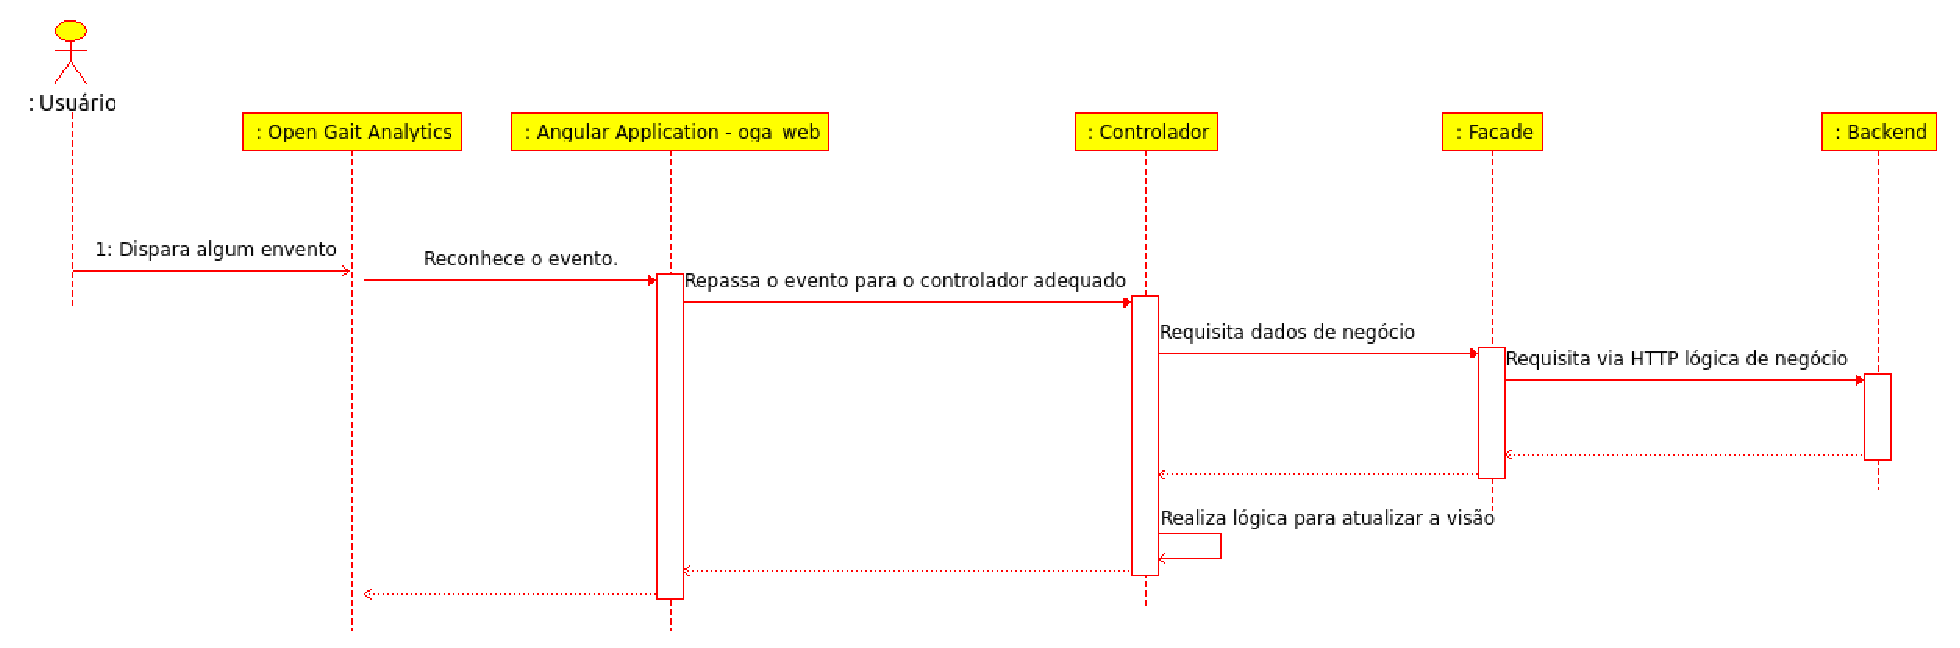
\includegraphics[width=17cm]{figuras/camada_web.eps}
	\caption{Camada \emph{web}.}
	\label{camda_web}
\end{figure}

Este esquema funciona da seguinte forma: O usuário usando seu \emph{browser}, acessa o \emph{site} do software. 
Ao realizar qualquer evento na aplicação, por exemplo, clicar num botão, ou selecionar um item em uma lista de seleção, a aplicação \emph{angularjs} detecta o evento e seleciona um componente de software chamado controlador. 
Existem vários destes controladores no sistema, cada evento do usuário é redirecionado para um que seja adequado.
No controlador é onde grande parte da programação acontece. 
Ele é associado a um \emph{template HTML}. 
Este template funciona como componente de apresentação para o usuário, e é o que o controlador manipula para mostrar informações ao usuário.
Quando o controlador precisa executar lógica de negócio, ou requisitar dados persistidos, ele deve chamar um componente do tipo \emph{Facade}. 
A aplicação \emph{web} roda no \emph{browser} do usuário e não persiste dados nem executa lógica de negócio. 
Este é um estilo arquitetural escolhido para o projeto.
A \emph{Facade} é um \emph{proxy} que se comunica com um \emph{backend} via HTTP no estilo \emph{REST} de comunicação via \emph{web}.

A Figura \ref{web_components}, mostra um exemplo de componentes escritos em \emph{JavaScript} respondendo a um evento disparado pelo usuário. 
Este evento poderia ser oriundo de um clique num botão ou na chamada de uma \emph{URL} específica. 
Depois de reconhecido o evento, no caso um pedido para ver a lista de pacientes, o componente \emph{PatientesCtrl} e o \emph{template patients.html} são carregado pelo \emph{framework AngularJS}. 
Neste momento o \emph{framework} acessa o componente \emph{PatientsFacade} através do seu método \emph{getPatients}. 
Este método invoca o método \emph{get} do componente \emph{\$HTTP} que faz parte do \emph{framework}.
Uma requisição é feita para o \emph{backend}, que retorna os dados no formato \emph{JSON}.
Finalmente, o \emph{framework} detecta a resposta e atualiza a tela para o usuário.

\begin{figure}[H]
	\centering
	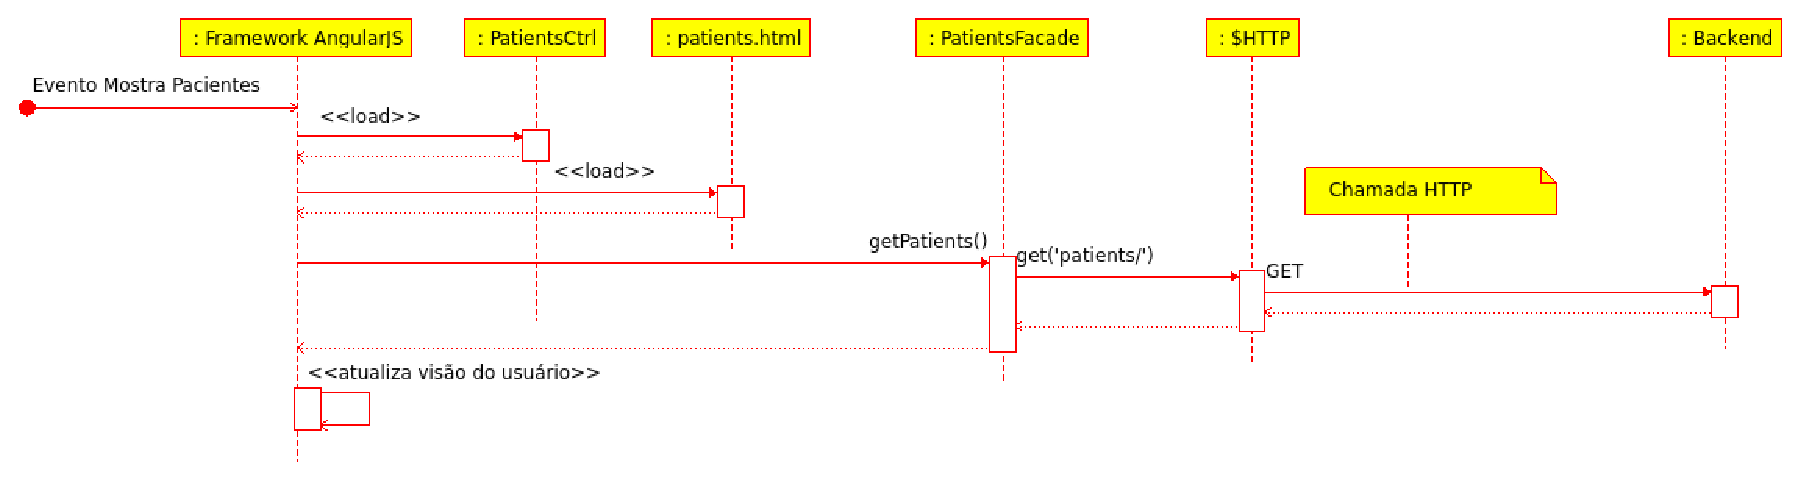
\includegraphics[width=17cm]{figuras/web_componentes.eps}
	\caption{Exemplo de componentes da camada \emph{web} funcionando juntos.}
	\label{web_components}
\end{figure}


\subsection{CAMADA \emph{REST WEB API}}

Esta é a camada responsável por expor toda a lógica de negócio e acesso a dados persistidos. Escolheu-se que esta camada fornece suas funções via \emph{web API} no estilo REST.
Uma das vantagens desta escolha é o alto desacoplamento, entre camada \emph{web} e lógica de negócio. 
Além disso, pode-se integrar mais facilmente a aplicação com outras, já que a lógica de negócio é toda exposta como \emph{API web}. 
Veja a seção \ref{servicos_rest} para um melhor entendimento deste estilo \emph{REST}.

\textbf{ORGANIZAÇÃO DO CÓDIGO FONTE}

\noindent
A Figura \ref{dir_api} mostra a configuração básica dos arquivos e diretórios da aplicação.

\begin{figure}[ht]
	\centering
	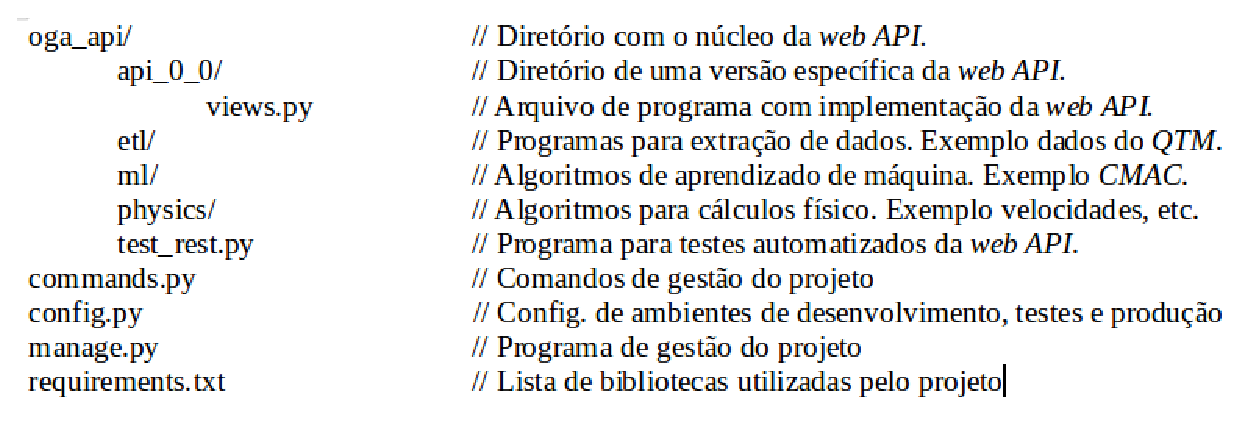
\includegraphics[width=15cm]{figuras/dir_api.eps}
	\caption{Organização do arquivos e diretórios da camada \emph{web API}.}
	\label{dir_api}
\end{figure}

A linguagem de programação \emph{Python} foi escolhida para implementar esta camada. Vários foram os motivos: a biblioteca \emph{Flask} para implementar a \emph{web API}, a biblioteca \emph{NumPy}, que é excelente para cálculos, comparável ao Matlab, a biblioteca \emph{Matplotlib} para criação de gráficos científicos, a baixa curva de aprendizado da linguagem, sua fama com desenvolvedores ao redor do mundo.

Para diminuir os problemas de ambientes, oriundos de um projeto complexo como este, optou-se por utilizar o programa \emph{virtualenv}. Este programa cria um ambiente \emph{python} virtual, baseado num arquivo de configuração. Isso faz com que todos os desenvolvedores envolvidos no projeto, possuam ambientes muito semelhantes.
Ao se clonar o projeto basta entrar no diretório da API e digitar o comando:
\lstset{language=bash}
\begin{lstlisting}[frame=single]
virtualenv env
\end{lstlisting}

Este comando irá criar uma diretório chamado \emph{env}. Para poder ativar o ambiente virtual é necessário o comado no unix:
\lstset{language=bash}
\begin{lstlisting}[frame=single]
. env/bin/activate
\end{lstlisting}

As bibliotecas necessárias a execução da aplicação estão listadas no arquivo \emph{requirements.txt}. Para instalá-las no novo ambiente virtual é necessário o comando:
\lstset{language=bash}
\begin{lstlisting}[frame=single]
pip install -r requirements.txt
\end{lstlisting}

Neste ponto, o código já pode ser editado e executado. Para facilitar um pouco as coisas, foi criado o programa \emph{manage.py}. Para rodar um servidor \emph{web} local respondendo na porta 5000, com fins de desenvolvimento, basta digitar o comando:
\lstset{language=bash}
\begin{lstlisting}[frame=single]
python manage.py runserver
\end{lstlisting}

Já para executar testes automatizados:
\lstset{language=bash}
\begin{lstlisting}[frame=single]
python manage.py test
\end{lstlisting}

Vale lembrar que o servidor \emph{MongoDB}, deve estar configurado, rodando e suas configurações editadas no arquivo \emph{config.py}.


\textbf{VISÃO ARQUITETURAL DA CAMADA \emph{REST WEB API}} 

\noindent
A Figura \ref{camada_api} mostra um \emph{blueprint} de como funciona e como deve ser desenvolvida esta camada.
\begin{figure}[ht]
	\centering
	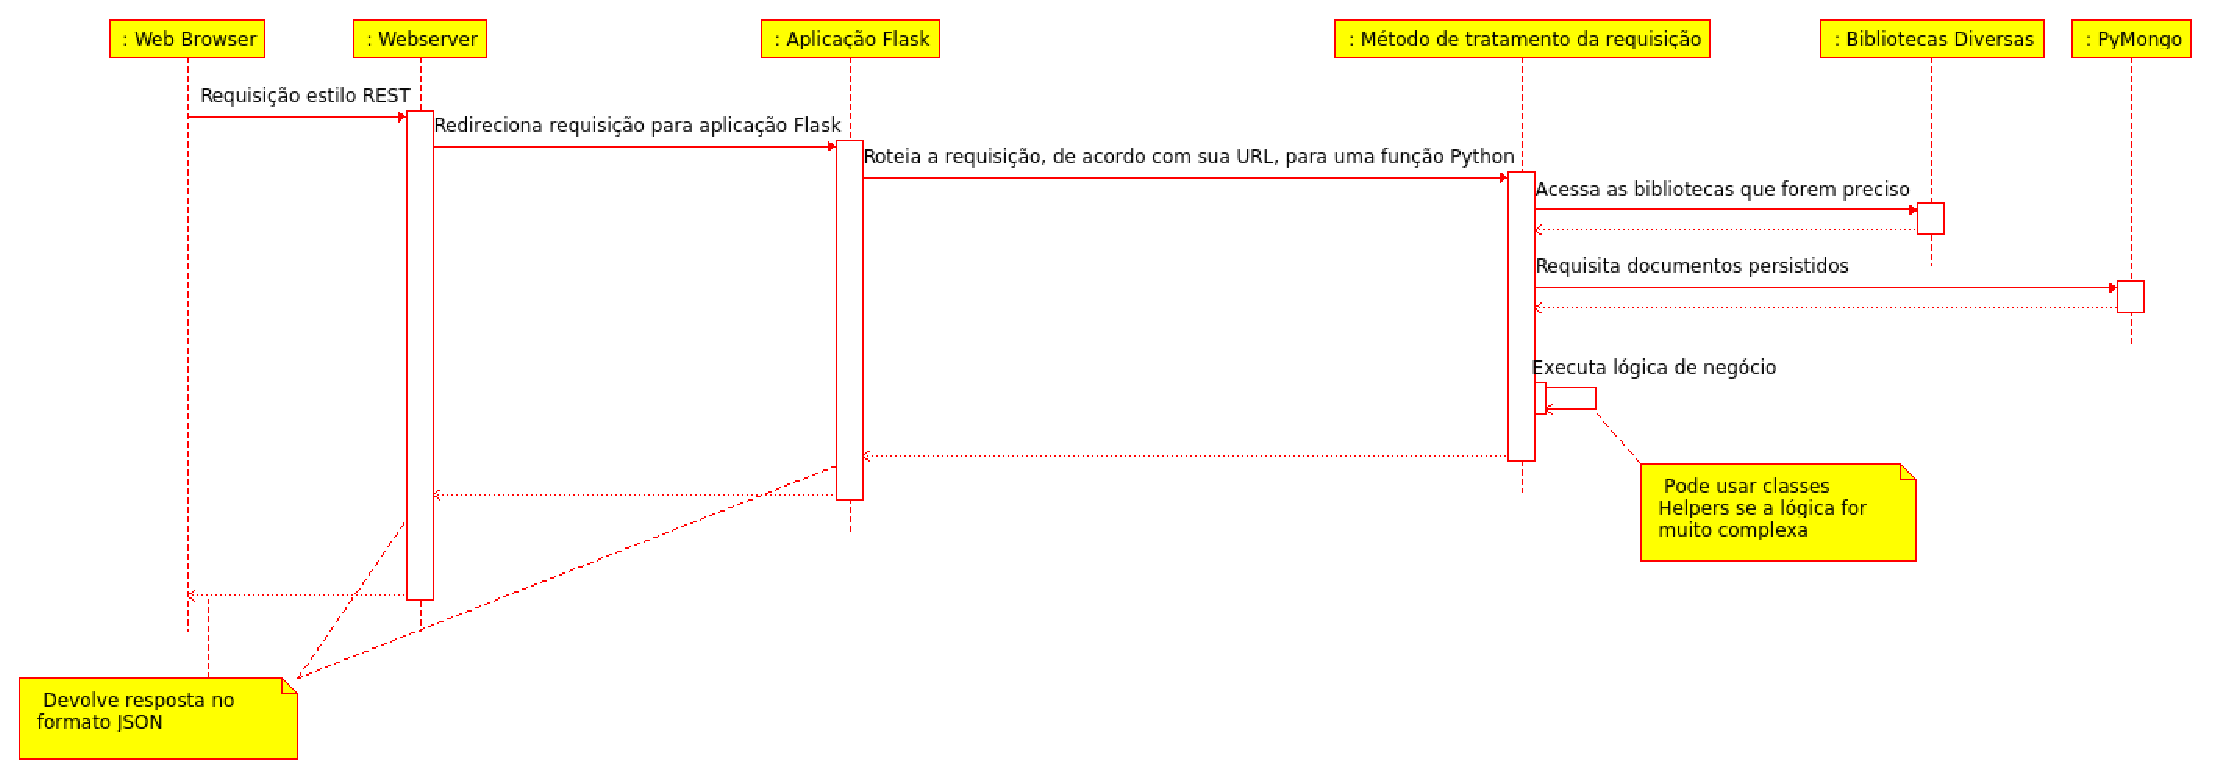
\includegraphics[width=15cm]{figuras/camada_api.eps}
	\caption{Camada \emph{REST WEB API}.}
	\label{camada_api}
\end{figure}

Tudo começa quando um \emph{browser web} faz uma requisição do tipo \emph{HTTP} a um servidor \emph{web}. 
O servidor \emph{web} identifica se a requisição é para a aplicação \emph{flask} do sistema em questão. 
Se for, esta requisição é repassada para a aplicação \emph{flask}. 
Agora as coisas começam a ficar mais interessantes. 
A aplicação \emph{flask} analisa a \emph{URL} da requisição, verifica o método da requisição e repassa os dados da requisição, num formato amigável ao \emph{python}, para uma função \emph{python}. 
Por padrão os parâmetros das requisições via método \emph{``GET"} são repassadas ao \emph{python} como \emph{string}. 
Para os demais métodos, padronizou-se receber o \emph{payload} da requisição \emph{HTTP}, como objetos JSON, que são facilmente convertidos para dicionários \emph{python}.

São nas funções \emph{python}, que tratam as requisições, que a lógica de negócio é executada. 
Aqui bibliotecas como a \emph{NumPy} podem ser chamadas, ou mesmo bibliotecas criadas pelos desenvolvedores da aplicação. 
É a partir deste ponto que dados podem ser acessados do banco de documentos pela biblioteca \emph{PyMongo}. 
Ao final da execução uma resposta é gerada no formato \emph{JSON} para que seja consumida pela camada \emph{web}.

A Figura \ref{webapi_componentes}, mostra um exemplo de componentes escritos em \emph{Python}, tratando uma requisição \emph{HTTP}, no caso uma chamada a \emph{URL http://<<myurl>>/patient}.
Depois que o servidor \emph{web} repassou a requisição para a aplicação que usa o \emph{framework Flask}, o \emph{framework} executa sua rotina de roteamento e descobre qual função \emph{Python}, contida no componente \emph{views},  deve ser executada, no caso a função \emph{get\_patients}.
Esta função acessa um objeto do tipo \emph{DataBase}, pertencente a biblioteca \emph{PyMongo}, e executa o método \emph{find} da coleção \emph{patients} pertencente ao \emph{DataBase}.
O resultado desta chamada são os dados contidos no banco de dados retornados no formato \emph{BSON}.
O componente \emph{json\_util}, da biblioteca \emph{PyMongo}, tem seu método \emph{dumps} chamado.
Este método converte os dados de \emph{BSON} para \emph{JSON}.
Finalmente, o \emph{framework Flask} responde a requisição.


\begin{figure}[ht]
	\centering
	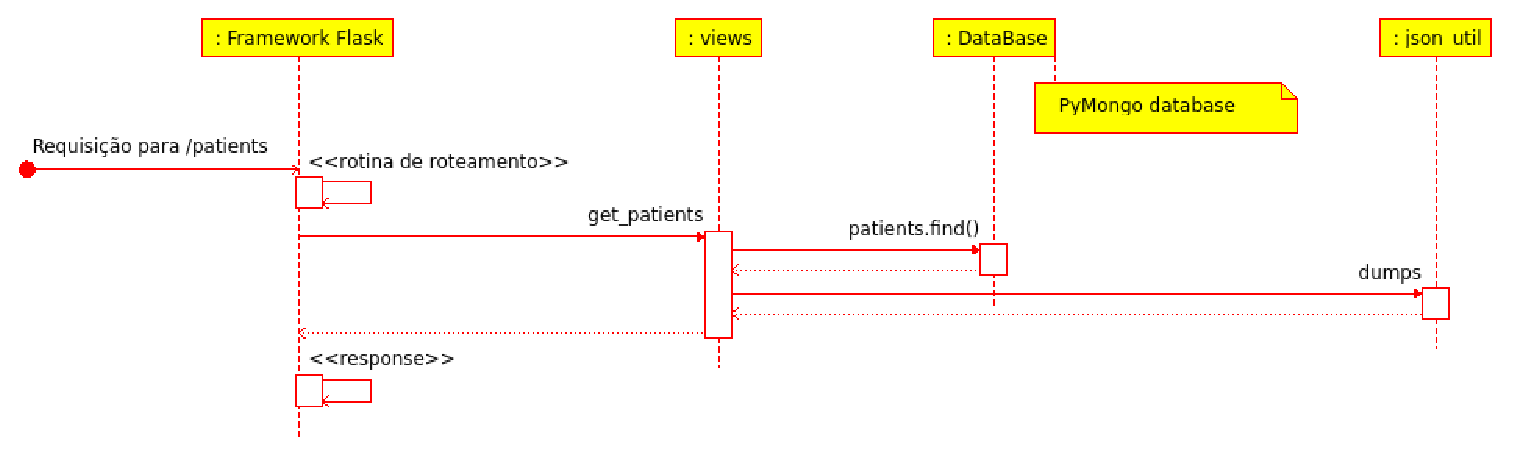
\includegraphics[width=17cm]{figuras/webapi_componentes.eps}
	\caption{Exemplo de requisição sendo tratada pela \emph{web api}.}
	\label{webapi_componentes}
\end{figure}

\subsection {CAMADA DE BASE DE DOCUMENTOS}

Para esta camada foi escolhido o banco de documentos \emph{MongoDB}, ver a seção \ref{mongodb_sec}. 
Há várias vantagens no uso desta tecnologia, mas a determinante foi a facilidade de uso e criação de estruturas de dados. 
No início do projeto, foi usado um banco de dados relacional e um \emph{framework} de mapeamento objeto-relacional. 
Devido a natureza altamente complexa dos dados, dados espaciais provindos de marcadores de superfície capturados por câmeras, eles são multidimensionais também. 
Sem dúvida isto ajudou a tornar possível criar esta primeira versão do software em tão pouco tempo.

A estrutura do banco da aplicação é mostrada na Figura \ref{mongo_oga}. 
O banco é composto por duas coleções: os dados dos pacientes na coleção \emph{patients} e os dados recuperados do \emph{QTM} \emph{positionals\_data}.

\begin{figure}[H]
	\centering
	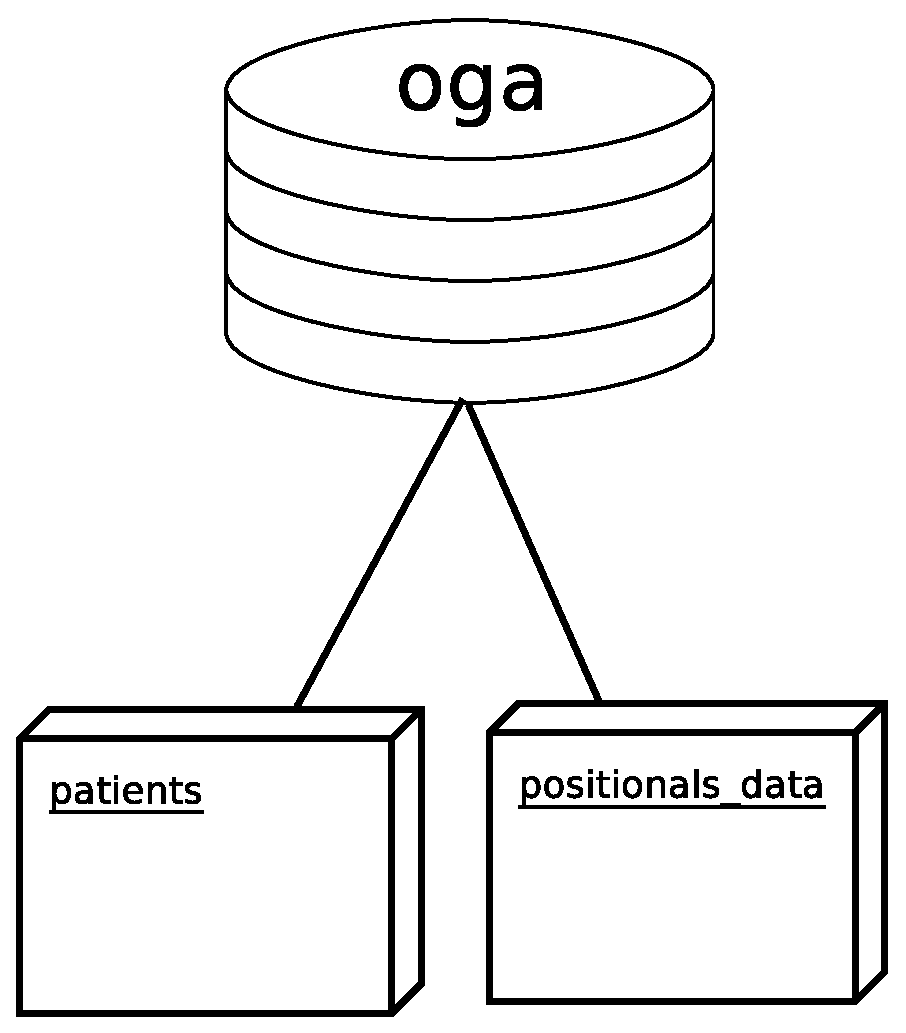
\includegraphics[width=5cm]{figuras/mongo_oga.eps}
	\caption{Banco de documentos da aplicação.}
	\label{mongo_oga}
\end{figure}

A Figura \ref{listagem2}  mostra um exemplo de documento da coleção \emph{patients}.
Já a Figura \ref{listagem3}  mostra um exemplo de documento da coleção \emph{positionals\_data}.

\begin{figure}[H]
	\centering
	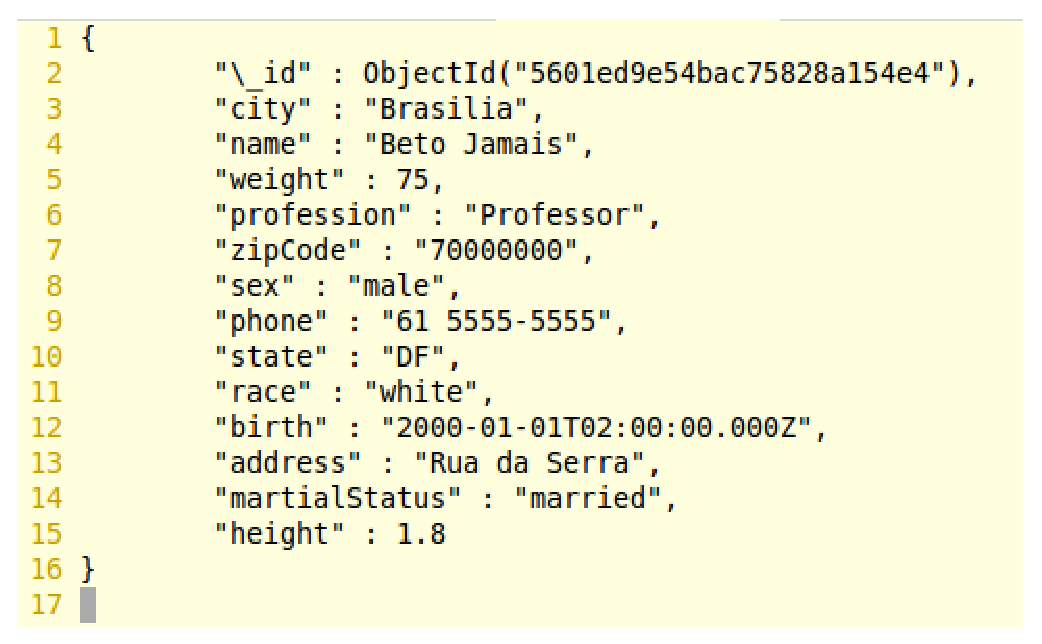
\includegraphics[width=10cm]{figuras/listagem2.eps}
	\caption{Documento da coleção \emph{patients}.}
	\label{listagem2}
\end{figure}

\begin{figure}[H]
	\centering
	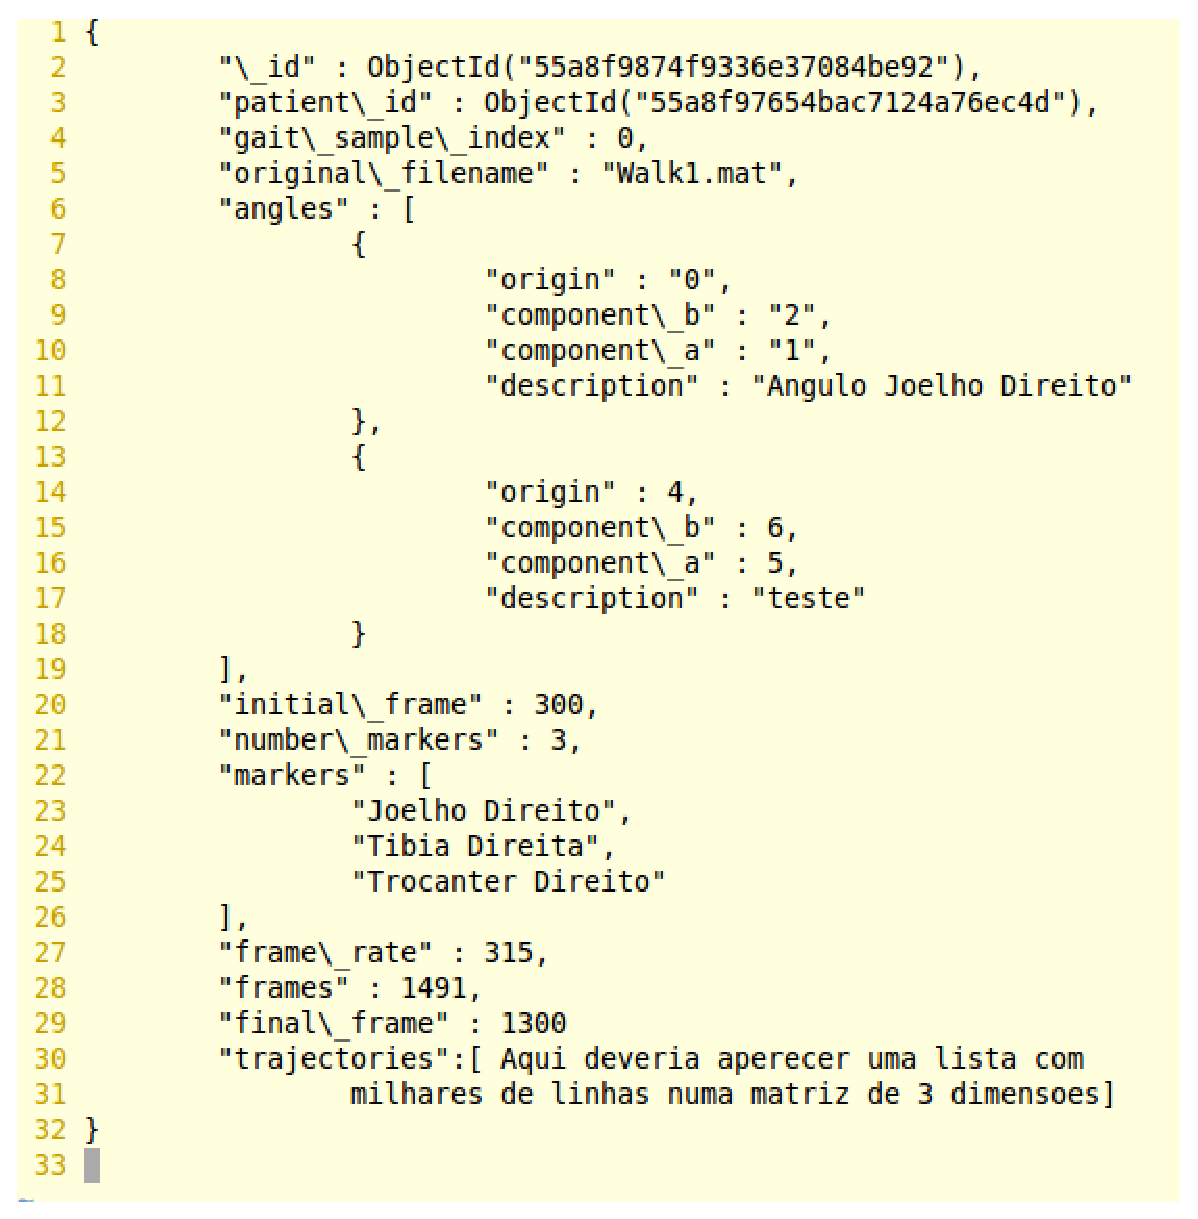
\includegraphics[width=10cm]{figuras/listagem3.eps}
	\caption{Documento da coleção \emph{positionals\_data}.}
	\label{listagem3}
\end{figure}




\begin{comment}
\section[FASES ESTUDO]{FASES DO ESTUDO}
\subsection[Coleta dos Dados]{\textbf{Coleta dos Dados}}
Os dados para o treinamento da RNA CMAC são dados cinemáticos, capturados através de \emph{motion capture}, utilizando-se de várias câmeras \emph{Qualisys Oqus MRI}, com marcadores passivos e pacote de software \emph(QTM 3.2) da \emph{Qualisys}. 
O sistema utilizado suporta até 74 canais, ou marcadores simultâneos.

O projeto no qual ocorreu a coleta foi aprovado pelo Comitê de Ética da Faculdade de Saúde da UnB, processo N11911/12 (ver Anexo \ref{anexo1}).

A Figura \ref{coleta_dados} mostra o processo para coleta de dados.

\begin{figure}[ht]
 \centering
 \includegraphics[width=4cm]{figuras/coleta_dados.eps}
 \caption{Fluxo de coleta de dados.}
 \label{coleta_dados}
\end{figure}

Primeiro deve-se definir o voluntário da coleta e determinar o dia para este processo. 
Além disso, também é necessário definir quais os pontos no corpo do voluntário devem ser mapeados. 
Também se devem distribuir os marcadores em várias posições ao longo das pernas. 
Como só a flexão e a extensão dos joelhos interessam para este trabalho, utilizam-se somente marcadores nas tíbias, joelhos e trocânteres das duas pernas.

O próximo passo se refere ao voluntário, isto é, ele deve repetir um ciclo de marcha confortável de aproximadamente 5 segundos, por 5 vezes na frente das câmeras.

Quanto aos dados, estes devem ser convertidos para formato adequado à linguagem \emph{Octave}, que é a mesma opção para converter para o \emph{MATLAB}. Esta opção é própria do \emph{QTM}. 
Além da conversão é necessário definir o nome de cada item na matriz de dados coletados. 
Cada coluna desta matriz representa um marcador, são estes pontos que devem ser nomeados. 
Por exemplo, coluna 1 igual ao trocânter direito. 
O número que o QTM atribui internamente ao marcador é a posição do marcador na matriz. 
Este número é chamado dentro do QTM de canal. 
Os dados trazem variáveis espaciais e o erro, com respeito à posição (X, Y, Z) dos marcadores.

A disposição que os dados obtidos neste processo se apresentam, é mostrado na Figura \ref{dados_qtm}.

\begin{figure}[ht]
 \centering
 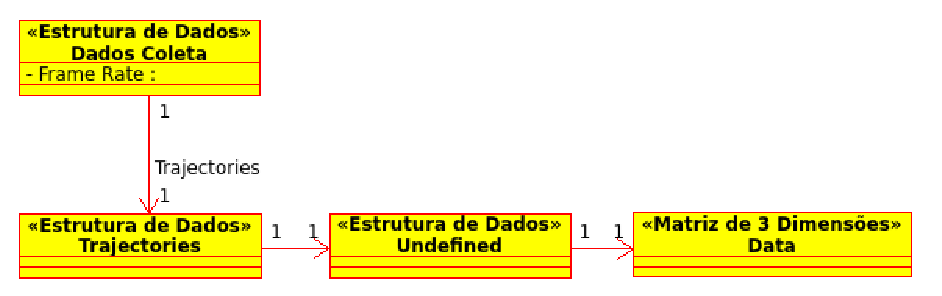
\includegraphics[width=15cm]{figuras/dados_qtm.eps}
 \caption{Dados disponibilizados pelo QTM.}
 \label{dados_qtm}
\end{figure}

Os dados que interessam são o \emph{Frame Rate} e o \emph{Data}.
São retornados vários dados, mas os de interesse para o projeto são os que estão na Figura \ref{dados_qtm}. 
O \emph{Frame Rate} é a taxa de coleta dos dados e está em segundos. 
A matriz de 3 dimensões está disposta da seguinte forma:
\begin{enumerate}
	\item A primeira dimensão é 74 e representa o número de canais do sistema de coleta;
	\item A segunda dimensão é 4 e representa a posição num plano 3D (X, Y, Z) do marcador, mais o erro;
	\item A terceira dimensão é número de frames coletados numa caminhada específica. Este número é variável.
\end{enumerate}



\subsection[Extração e transformação dos dados]{\textbf{Extração e transformação dos dados}}
Com os dados necessários disponibilizados no formato adequado é possível fazer os cálculos de angulações, velocidades angulares e acelerações angulares dos joelhos. Os casos de uso para esta fase são:
\begin{figure}[ht]
	\centering
	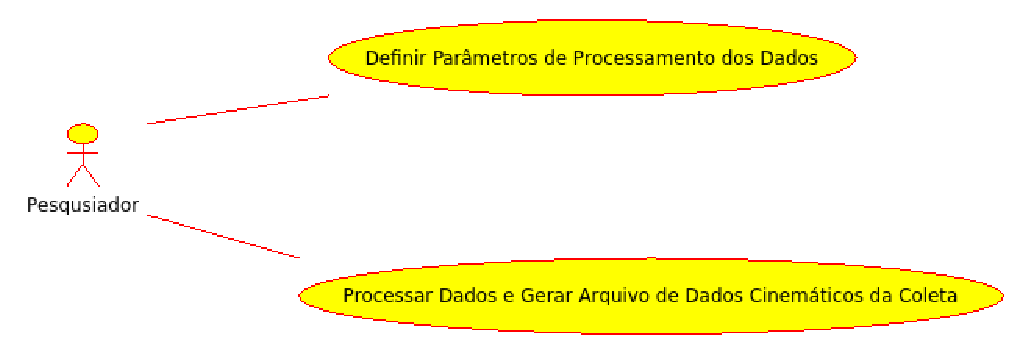
\includegraphics[width=15cm]{figuras/extracao_coleta.eps}
	\caption{Caso de uso para extração e transformação de dados}
	\label{extracao_coleta}
\end{figure}

O caso de uso Definir Parâmetros de Processamento dos Dados, definido na Figura \ref{extracao_coleta}, consiste em se definir os dados necessários para que depois seja possível processar os dados coletados. 
Estes dados são os definidos na Figura \ref{estrutura_dados}. 
O valor dos 6 primeiros atributos da estrutura de dados Configuração do Processamento, são os canais usados no QTM para tais marcadores.
\begin{figure}[ht]
	\centering
	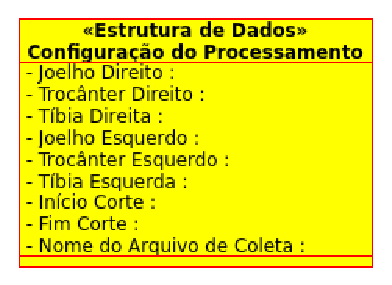
\includegraphics[width=7.5cm]{figuras/estrutura_dados.eps}
	\caption{Dados para processamento da coleta.}
	\label{estrutura_dados}
\end{figure}

O caso de uso Processar Dados e Gerar Arquivos de Dados Cinemáticos, definido na Figura \ref{extracao_coleta}, da coleta deve obedecer o processo da Figura \ref{tratamento_dados}.
\begin{figure}[ht]
	\centering
	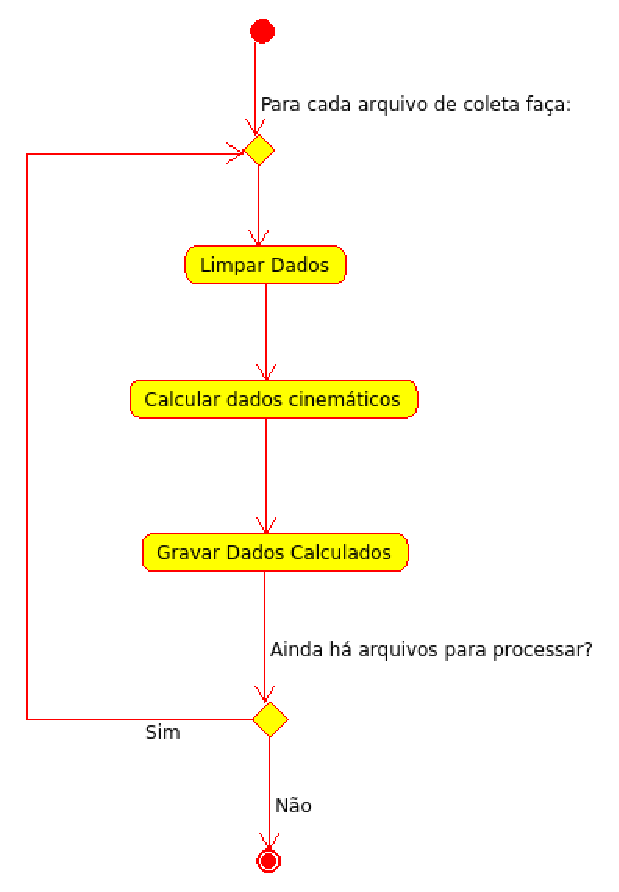
\includegraphics[width=10cm]{figuras/tratamento_dados.eps}
	\caption{Processo de tratamento dos dados.}
	\label{tratamento_dados}
\end{figure}

A limpeza dos dados consiste em retirar os dados desnecessários, como marcadores não desejados e retirada de frames do início e/ou final de um arquivo de coleta, que não estejam no ciclo de marcha confortável. 

Os cálculos realizados devem ser as velocidades instantâneas, velocidades angulares e acelerações angulares. 
Velocidades instantâneas dos joelhos são calculadas conforme a Equação \ref{velocidade}.
\begin{equation}
	\label{velocidade}
	\vec{\nu} = (\vec{a}-\vec{b})/t 
\end{equation}

A variável $\vec{a}$  é a posição (X, Y, Z) do joelho em uma determinada leitura sequencial dos dados coletados. 
A variável $\vec{b}$ é a próxima posição (X, Y, Z) da sequência. $t$ é o \emph{frame rate} definido nos dados da coleta.

Para o cálculo das angulações dos joelhos, primeiro os marcadores destes devem ser transladados para uma origem, assim é possível se usar a Equação 5 como descrita em \citeonline{Edwards2006}. 
Para tal, usam-se as Equações \ref{trocanter}, \ref{joelho} e \ref{tibia}.
\begin{equation}
	\label{trocanter}
	\vec{t_{r0}} = \vec{t_r} - \vec{j}
\end{equation}
\begin{equation}
	\label{joelho}
	\vec{j_0} = \vec{j} - \vec{j}
\end{equation}
\begin{equation}
	\label{tibia}
	\vec{t_{b0}} = \vec{t_b} - \vec{j}
\end{equation}

$\vec{t_{r0}}$ é o vetor que representa a posição de um trocânter $\vec{t_r}$, transladado para a nova origem.
$\vec{j}$ é vetor da posição do joelho.
$\vec{j_0}$ é a nova origem, que nada mas é que o joelho transladado para a posição $(0,0,0)$. 
$\vec{t_{b0}}$ é a posição da tíbia $\vec{t_b}$ transladada para a origem.
A translação de vetores é documentada em \citeonline{Poole2011}.

Agora que se tem os pontos transladados para uma origem, pode-se usar a Equação \ref{ang_joe} para o cálculo do ângulo $\theta$ do joelho.
\begin{equation}
	\label{ang_joe}
	\theta =
		cos^{-1} 
		\frac
		{
			\vec{t_{r0}} \cdot \vec{t_{b0}}
		}
		{
			\left \| \vec{t_{r0}} \right \|
			\cdot
			\left \| \vec{t_{b0}} \right \|
		}
\end{equation}

O operador $\left \| \right \|$ é o cálculo da distância euclidiana, ou norma. Pode ser calculado, segundo \citeonline{Poole2011}, de acordo com a Equação \ref{norma}. Resumindo, é a raiz quadrada do produto interno de um vetor.
\begin{equation}
	\label{norma}
	\left \| \vec{u} \right \| = \sqrt{\vec{u}\cdot\vec{u}}
\end{equation}

A velocidade angular $\omega$ do joelho é calculada a partir da Equação \ref{vel_ang}.
\begin{equation}
	\label{vel_ang}
	\omega = (\theta_1 - \theta_2) / t
\end{equation}

A variável $\theta_1$ é o ângulo de um joelho num determinado frame. A variável $\theta_2$ é exatamente o ângulo do próximo frame. A variável $t$ é o \emph{frame rate}, oriundo dos dados da coleta.


A última etapa deste processo é a gravação dos dados para que possam ser usados pela RNA CMAC. 
Estes dados devem ser gravados num arquivo em formato texto. 
As linhas neste arquivo equivalem aos \emph{frames}. 
Cada coluna equivale às informações, na ordem em que aparecem, da estrutura de dados descrita na Figura \ref{dados_cinematicos}. 
\begin{figure}[ht]
	\centering
	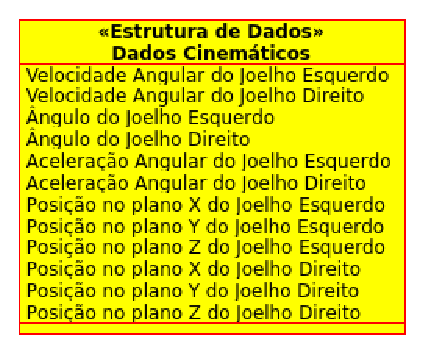
\includegraphics[width=7.5cm]{figuras/dados_cinematicos.eps}
	\caption{Dados Cinemáticos da Marcha}
	\label{dados_cinematicos}
\end{figure}

\subsection[Construção de uma RNA CMAC]{\textbf{Construção}}
\subsubsection{Modelo Geral}

A RNA CMAC proposta para este trabalho é resumida na Figura \ref{camac_resumida}.

\begin{figure}[ht]
	\centering
	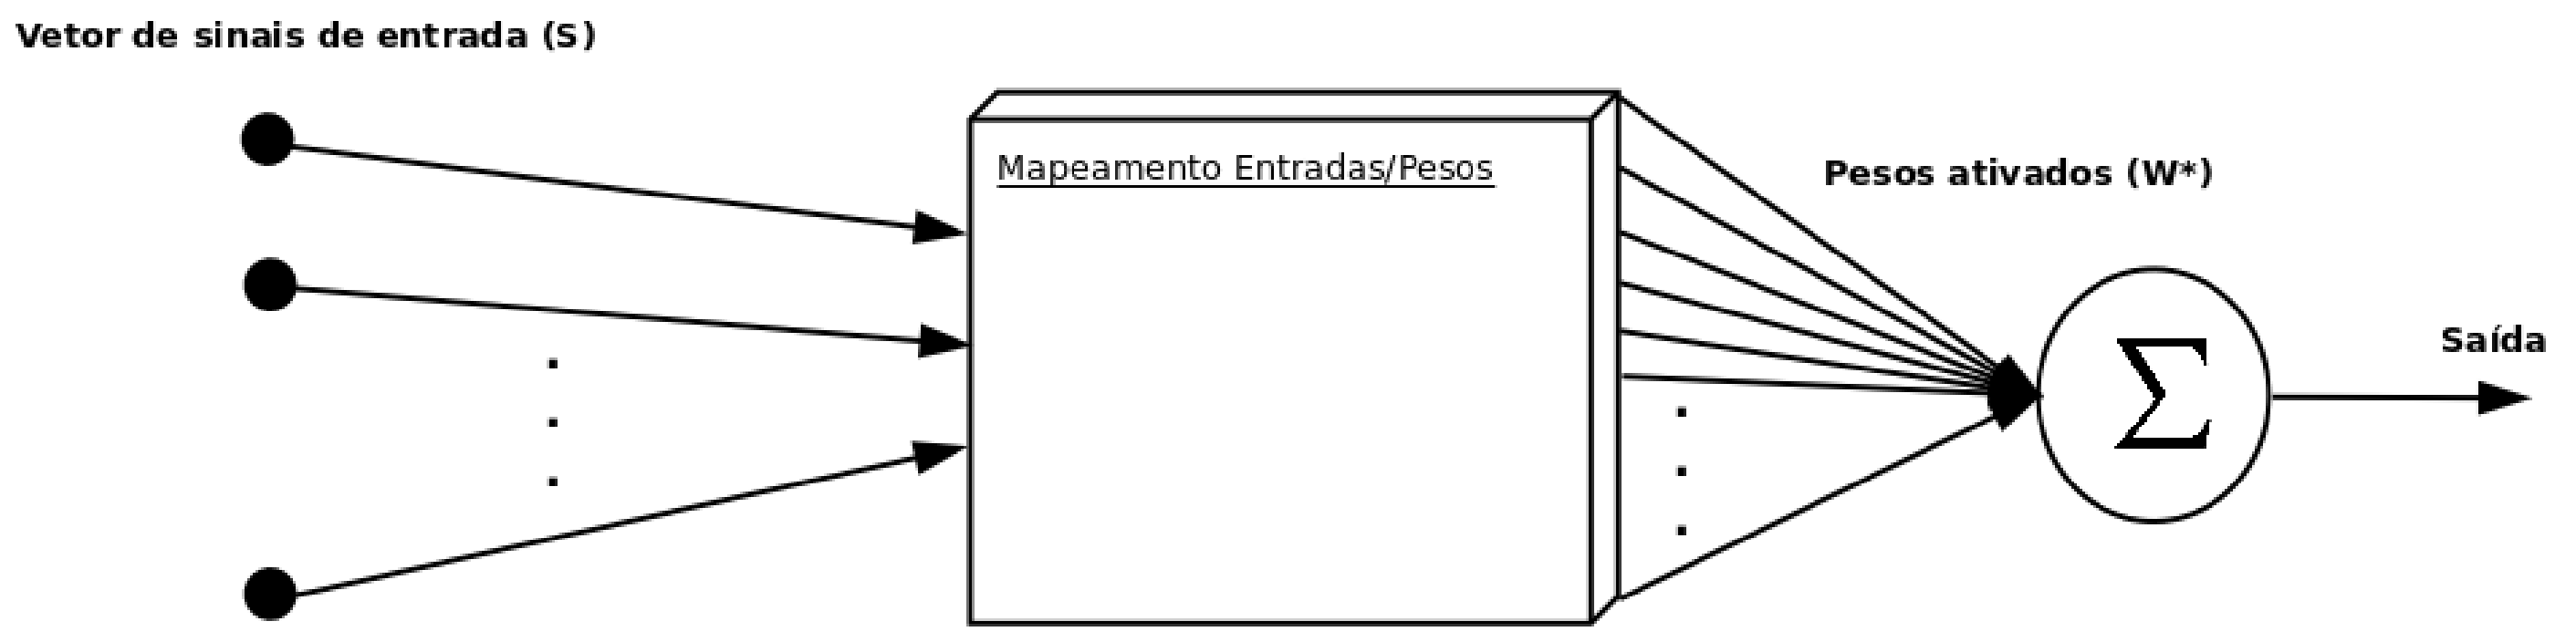
\includegraphics[width=15cm]{figuras/cmac_resumida.eps}
	\caption{CMAC resumida.}
	\label{camac_resumida}
\end{figure}

A variável $S$ é o vetor de sinais de entrada. 
Esses sinais são passados para um processo de mapeamento entre a entrada e um conjunto de pesos. 
Depois apenas os pesos ativados participam da somatória que é o sinal de saída. 

Para se calcular a saída da rede, primeiramente define-se o número de pesos $NW*$ a serem ativados.

O segundo passo é definir os possíveis valores para cada item do vetor de entradas $S$. A isto chama-se quantização. Por exemplo, se o primeiro item $s1$ de $S$ aceita valores entre $-1$ até $1$ e se quer $5$ valores possíveis, quantiza-se $s1$ conforme a Figura \ref{quantizacao}.
\begin{figure}[ht]
	\centering
	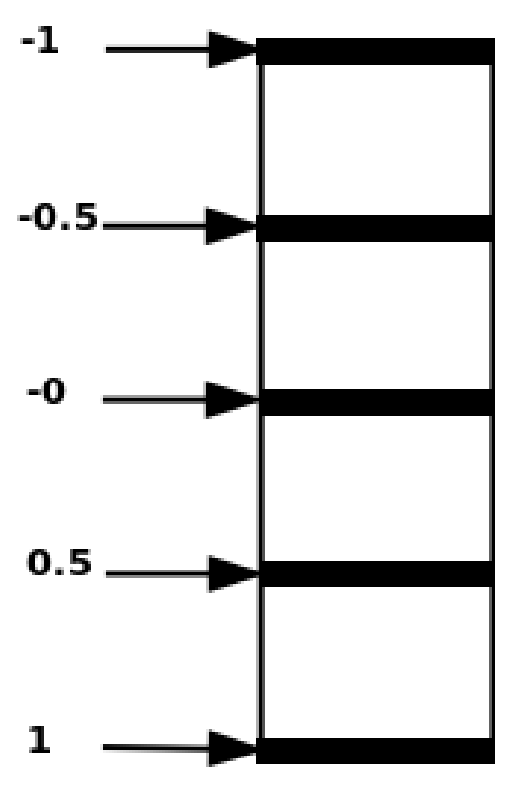
\includegraphics[width=5cm]{figuras/quatizacao.eps}
	\caption{Quantização de $s1$}
	\label{quantizacao}
\end{figure}

Isto significa que quaisquer que sejam os valores de $s1$ os mesmos devem ser convertidos para $-1$, $-0,5$, $0$, $0,5$ e $1$. 
Por exemplo, se o valor de s1 for $0,75$, será convertido para o valor $1$, se for $-0,75$ será o valor $0$ e se for $0,25$ será o valor $0,5$. À discretização dá-se o nome de resolução da CMAC.

O próximo passo é criar uma tabela para cada um dos sinais discretizados de entrada do vetor $S$.
Supondo que o vetor $S$ possui 2 sinais de entrada $s1$ e $s2$ e um número de ativações $NW*$ igual a 3, cria-se Tabela \ref{map_s1} e a Tabela \ref{map_s2}. 
Para facilitar o entendimento, irá se considerar os valores de $s1$ iguais aos inteiros de 1 até 6 e os valores de s2 iguais aos inteiros de 1 até 4.
\begin{table}[htb]
	\IBGEtab{%
		\caption{Mapeamento de $s1$}%
		\label{map_s1}
	}
	{%
		\begin{tabular}{cc}
			\toprule
			\textbf{Valores de $s1$} & \textbf{Mapeamento $m1$} \\
			\midrule
			1	&	0, 1, 2	\\
			\midrule
			2	&	3, 1, 2	\\
			\midrule
			3	&	3, 4, 3	\\
			\midrule
			4	&	3, 4, 5	\\
			\midrule
			5	&	6, 4, 6	\\
			\midrule
			6	&	6, 7, 5	\\
			\bottomrule
		\end{tabular}%
	}
	{%
		\fonte{Produzido pelo autor.}%
	}
\end{table}

\begin{table}[htb]
	\IBGEtab{%
		\caption{Mapeamento de $s2$}%
		\label{map_s2}
	}
	{%
		\begin{tabular}{cc}
			\toprule
			\textbf{Valores de $s2$} & \textbf{Mapeamento $m2$} \\
			\midrule
			1	&	0, 1, 2	\\
			\midrule
			2	&	3, 1, 2	\\
			\midrule
			3	&	3, 4, 3	\\
			\midrule
			4	&	3, 4, 5	\\
			\bottomrule
		\end{tabular}%
	}
	{%
		\fonte{Produzido pelo autor.}%
	}
\end{table}

Estas tabelas são criadas da seguinte forma:
O mapeamento consiste num número de itens igual a $NW*$, 3 no caso.
Este número é o número de pesos a serem ativados.
Para a primeira linha de cada uma das tabelas, atribui-se uma sequência de 3 valores inteiros começando com 0.
A próxima linha deve conter o próximo valor da sequência, 3, como primeiro item do mapeamento e continuar com os demais itens iguais aos da linha anterior. 
Na próxima linha, substitui-se o segundo item de mapeamento pelo próximo número da sequência, 4, mantendo-se os demais itens e assim sucessivamente.

Depois de mapeado cada valor de cada item de entrada, deve-se combinar os mapeamentos de acordo com a Tabela \ref{map_w}.
\begin{table}[htb]
	\IBGEtab{%
		\caption{Mapeamento para os pesos $W$}%
		\label{map_w}
	}
	{%
		\begin{tabular}{ccccc}
			\toprule
			\begin{tabular}{c}
				\textbf{$s2$}	\\
				\textbf{$s1$}	\\
			\end{tabular} 
			& \textbf{1} & \textbf{2} & \textbf{3} & \textbf{4} \\
			\midrule
			\textbf{1}	& 1 & 2 & 3 & 4 \\
			\bottomrule
		\end{tabular}%
	}
	{%
		\fonte{Produzido pelo autor.}%
	}
\end{table}

\end{comment}


\input{cap4/visibilidade}

\bookmarksetup{startatroot} 
\postextual

\renewcommand{\bibname}{\textbf{REFERÊNCIAS BIBLIOGRÁFICAS}} % Altera o nome da Referêcia para Referêcia Bibliográfica
\bibliography{bibliografia}
\printindex
\end{document}